\label{kap:stereometrie}
\mathquote{Let no one ignorant of geometry enter.}{nápis nad vchodem do Platónovy Akademie (podle legendy)}

Stereometrie je geometrie v prostoru. Všechno, co jsme se naučili v rovině, platí dál, jen se objeví jedna nová dimenze a s ní nové situace. Například dvě přímky, které se neprotínají, a přesto nejsou rovnoběžné. V první části kapitoly se podíváme na vzájemné polohy a vzdálenosti útvarů v prostoru, ve druhé na tělesa, jejich objemy a povrchy.

\section{Polohové vlastnosti}

\begin{definitionbox}
  \textbf{Vzájemná poloha dvou přímek v prostoru}:
  \begin{itemize}
    \item \textbf{totožné},
    \item \textbf{rovnoběžné různé}: leží v jedné rovině a nemají společný bod,
    \item \textbf{různoběžné}: mají právě jeden společný bod (a tedy leží v jedné rovině),
    \item \textbf{mimoběžné}: \textbf{neleží v jedné rovině}, nemají společný bod a nejsou rovnoběžné.
  \end{itemize}

  \textbf{Vzájemná poloha přímky a roviny}: přímka \textbf{leží v rovině}, je s ní \textbf{rovnoběžná} (nemá s ní společný bod), nebo je s ní \textbf{různoběžná} (protíná ji v jednom bodě, tzv. průsečíku).

  \textbf{Vzájemná poloha dvou rovin}: \textbf{totožné}, \textbf{rovnoběžné různé}, nebo \textbf{různoběžné} (protínají se v přímce, tzv. průsečnici).
\end{definitionbox}

Mimoběžky jsou ta novinka, kvůli které stereometrie stojí za samostatnou kapitolu. V rovině se dvě nerovnoběžné přímky vždy protnou. V prostoru se mohou minout. Představte si dálniční most přes jinou dálnici: silnice nahoře a dole se nikdy nepotkají a přitom nejsou rovnoběžné.

\begin{definitionbox}
  \textbf{Užitečná kritéria}:
  \begin{itemize}
    \item Přímka je rovnoběžná s rovinou, pokud je rovnoběžná s nějakou přímkou ležící v této rovině.
    \item Dvě roviny jsou rovnoběžné, pokud jedna obsahuje dvě různoběžky rovnoběžné s druhou rovinou.
    \item Pokud dvě rovnoběžné roviny protneme třetí rovinou, jsou průsečnice \textbf{rovnoběžné}.
    \item Přímka je kolmá k rovině, pokud je kolmá ke dvěma různoběžkám této roviny.
  \end{itemize}
\end{definitionbox}

V dalších příkladech budeme pracovat s krychlí $ABCDEFGH$, kde $ABCD$ je dolní podstava, $EFGH$ horní podstava a hrana $AE$ je svislá (bod $E$ je nad $A$, $F$ nad $B$ a tak dále).

\begin{center}
  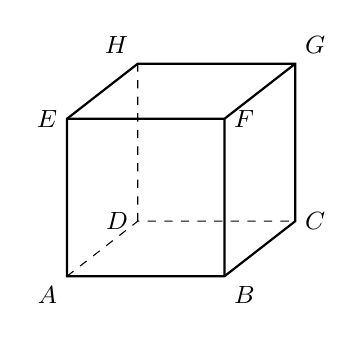
\begin{tikzpicture}[scale=2, x={(1cm,0cm)}, y={(0.45cm,0.35cm)}, z={(0cm,1cm)}]
    \coordinate (A) at (0,0,0); \coordinate (B) at (1,0,0); \coordinate (C) at (1,1,0); \coordinate (D) at (0,1,0);
    \coordinate (E) at (0,0,1); \coordinate (F) at (1,0,1); \coordinate (G) at (1,1,1); \coordinate (H) at (0,1,1);
    \draw[thick] (A) -- (B) -- (C) -- (G) -- (H) -- (E) -- cycle;
    \draw[thick] (B) -- (F) -- (G) (E) -- (F);
    \draw[dashed] (A) -- (D) -- (C) (D) -- (H);
    \node[below left] at (A) {\small $A$}; \node[below right] at (B) {\small $B$}; \node[right] at (C) {\small $C$}; \node[left] at (D) {\small $D$};
    \node[left] at (E) {\small $E$}; \node[right] at (F) {\small $F$}; \node[above right] at (G) {\small $G$}; \node[above left] at (H) {\small $H$};
  \end{tikzpicture}
\end{center}

\begin{example}
  V krychli $ABCDEFGH$:
  \begin{itemize}
    \item $AB$ a $HG$ jsou rovnoběžné (obě jsou rovnoběžné s $DC$),
    \item $AB$ a $BF$ jsou různoběžné (průsečík $B$), dokonce kolmé,
    \item $AB$ a $CG$ jsou mimoběžné. Neprotínají se, nejsou rovnoběžné a žádná rovina je neobsahuje obě,
    \item $AB$ a rovina $EFG$ jsou rovnoběžné (protože $AB\parallel EF$),
    \item rovina $ABF$ (přední stěna) a rovina $BCG$ (pravá stěna) jsou různoběžné s průsečnicí $BF$.
  \end{itemize}
\end{example}

\begin{problem}
  Určete vzájemnou polohu v krychli $ABCDEFGH$:
  \begin{enumerate}[label=(\alph*)]
    \item přímek $AG$ a $BH$,
    \item přímek $AC$ a $FH$,
    \item přímek $BD$ a $EG$,
    \item přímek $BD$ a $CG$,
    \item přímky $AC$ a roviny $EFG$,
    \item rovin $ACG$ a $BDH$.
  \end{enumerate}
\end{problem}

\begin{solution}
  \begin{enumerate}[label=(\alph*)]
    \item Různoběžné, jsou to tělesové úhlopříčky a protínají se ve středu krychle.
    \item Mimoběžné. Na první pohled vypadají jako rovnoběžky, protože jsou to úhlopříčky protilehlých stěn. Jenže $FH$ je rovnoběžná s $BD$, ne s $AC$. A protože leží v různých rovnoběžných rovinách, nemohou se ani protnout. Tohle je přesně ten typ chyby, který se v prostoru dělá nejčastěji.
    \item Mimoběžné. Jejich průměty do podstavy jsou dvě různé úhlopříčky čtverce, které se protínají, ale přímky samotné jsou v různých výškách.
    \item Mimoběžné. Svislá přímka $CG$ protíná rovinu podstavy v bodě $C$, který na $BD$ neleží.
    \item Rovnoběžné, $AC\parallel EG$.
    \item Různoběžné, jejich průsečnicí je svislá přímka procházející středy podstav.
  \end{enumerate}
\end{solution}

\subsection{Řezy těles}

Řez tělesa rovinou je průnik tělesa s rovinou. U krychle je to mnohoúhelník, jehož strany leží ve stěnách krychle. Při konstrukci řezu se používají dvě pravidla:
\begin{enumerate}
  \item Dva body roviny řezu, které leží ve stejné stěně, spojíme úsečkou.
  \item Roviny řezu protínají \textbf{rovnoběžné} stěny v \textbf{rovnoběžných} úsečkách.
\end{enumerate}
Pokud to nestačí, prodloužíme úsečku řezu ve stěně až k průsečíku s přímkou hrany a tím získáme další bod roviny řezu v sousední stěně.

\begin{example}
  Řez krychle rovinou $BDE$ je rovnostranný trojúhelník $BDE$ se stranou $a\sqrt{2}$, protože všechny jeho strany jsou stěnové úhlopříčky. Řez rovinou procházející středy hran $AB$, $BC$, $CG$, $GH$, $HE$ a $EA$ je dokonce \textbf{pravidelný šestiúhelník}. Tato rovina je kolmá na tělesovou úhlopříčku $DF$ a prochází středem krychle.
  \begin{center}
    \begin{tikzpicture}[scale=2.1, x={(1cm,0cm)}, y={(0.45cm,0.35cm)}, z={(0cm,1cm)}]
      \coordinate (A) at (0,0,0); \coordinate (B) at (1,0,0); \coordinate (C) at (1,1,0); \coordinate (D) at (0,1,0);
      \coordinate (E) at (0,0,1); \coordinate (F) at (1,0,1); \coordinate (G) at (1,1,1); \coordinate (H) at (0,1,1);
      \fill[colorofwisdom!25] (0.5,0,0) -- (1,0.5,0) -- (1,1,0.5) -- (0.5,1,1) -- (0,0.5,1) -- (0,0,0.5) -- cycle;
      \draw[thick, colorofwisdom] (0.5,0,0) -- (1,0.5,0) -- (1,1,0.5) -- (0.5,1,1) -- (0,0.5,1) -- (0,0,0.5) -- cycle;
      \draw[thick] (A) -- (B) -- (C) -- (G) -- (H) -- (E) -- cycle;
      \draw[thick] (B) -- (F) -- (G) (E) -- (F);
      \draw[dashed] (A) -- (D) -- (C) (D) -- (H);
      \node[below left] at (A) {\small $A$}; \node[below right] at (B) {\small $B$}; \node[right] at (C) {\small $C$}; \node[left] at (D) {\small $D$};
      \node[left] at (E) {\small $E$}; \node[right] at (F) {\small $F$}; \node[above right] at (G) {\small $G$}; \node[above left] at (H) {\small $H$};
    \end{tikzpicture}
  \end{center}
  Ověřit to můžeme v souřadnicích. Pro krychli s hranou $1$ a $A = [0, 0, 0]$ leží všech šest středů hran v rovině $x - y + z = \frac{1}{2}$ (dosaďte si) a vzdálenost každých dvou sousedních je $\frac{\sqrt{2}}{2}$.
\end{example}

\section{Metrické vlastnosti}

\begin{definitionbox}
  \textbf{Vzdálenosti}:
  \begin{itemize}
    \item \textbf{Vzdálenost bodu od přímky} (roviny) je vzdálenost bodu od jeho kolmého průmětu (paty kolmice) na přímku (rovinu).
    \item \textbf{Vzdálenost rovnoběžných přímek} (rovin, přímky a s ní rovnoběžné roviny) je vzdálenost libovolného bodu jednoho útvaru od druhého útvaru.
    \item \textbf{Vzdálenost mimoběžek} je délka jejich \textbf{osy}, tedy úsečky, která je kolmá na obě mimoběžky a spojuje je.
  \end{itemize}

  \textbf{Odchylky}:
  \begin{itemize}
    \item \textbf{Odchylka dvou přímek} je velikost ostrého (nebo pravého) úhlu, který svírají. U mimoběžek je to odchylka různoběžek rovnoběžných s nimi, vedených jedním bodem.
    \item \textbf{Odchylka přímky a roviny} je odchylka přímky a jejího kolmého průmětu do roviny.
    \item \textbf{Odchylka dvou rovin} je odchylka přímek, které v obou rovinách leží a jsou kolmé na průsečnici v jednom jejím bodě.
  \end{itemize}
  Odchylky jsou vždy z intervalu $[0^\circ, 90^\circ]$.
\end{definitionbox}

Metrické úlohy v prostoru se skoro vždy řeší stejně. Najdeme vhodný pravoúhlý trojúhelník, který leží v nějaké rovině, a použijeme Pythagorovu větu nebo goniometrické funkce z kapitoly~\ref{kap:goniometrie}. Celý trik je v tom, ten trojúhelník najít.

\begin{example}
  V krychli o hraně $a$:
  \begin{itemize}
    \item \textbf{stěnová úhlopříčka}: $|AC| = \sqrt{a^2 + a^2} = a\sqrt{2}$,
    \item \textbf{tělesová úhlopříčka}: trojúhelník $ACG$ je pravoúhlý s pravým úhlem u $C$ (hrana $CG$ je kolmá na celou podstavu), takže $|AG| = \sqrt{2a^2 + a^2} = a\sqrt{3}$,
    \item \textbf{odchylka tělesové úhlopříčky od podstavy}: je to úhel $GAC$, pro který $\tg\varphi = \frac{|CG|}{|AC|} = \frac{a}{a\sqrt{2}} = \frac{\sqrt{2}}{2}$, tedy $\varphi\approx 35{,}26^\circ$,
    \item \textbf{odchylka přímek $AF$ a $AH$} (stěnové úhlopříčky ze stejného vrcholu): trojúhelník $AFH$ má všechny strany stěnové úhlopříčky, je tedy rovnostranný a odchylka je $60^\circ$,
    \item \textbf{vzdálenost mimoběžek $AB$ a $CG$}: úsečka $BC$ je kolmá na obě, takže vzdálenost je $a$.
  \end{itemize}
\end{example}

\begin{problem}
  \begin{enumerate}[label=(\alph*)]
    \item Kvádr má rozměry $3$, $4$ a $12$. Jak dlouhá je jeho tělesová úhlopříčka?
    \item V krychli o hraně $a$ určete vzdálenost bodu $A$ od přímky $FH$.
    \item V krychli o hraně $a$ určete odchylku rovin $ABC$ a $ABG$.
    \item V pravidelném čtyřbokém jehlanu má podstava hranu $6$ a výška je $4$. Určete délku boční hrany a odchylku boční stěny od podstavy.
  \end{enumerate}
\end{problem}

\begin{solution}
  \begin{enumerate}[label=(\alph*)]
    \item $\sqrt{9 + 16 + 144} = 13$.
    \item Trojúhelník $AFH$ je rovnostranný se stranou $a\sqrt{2}$, vzdálenost $A$ od $FH$ je jeho výška: $\frac{\sqrt{3}}{2}a\sqrt{2} = \frac{\sqrt{6}}{2}a$.
    \item Průsečnice je $AB$. V rovině $ABC$ je na ni kolmá $BC$, v rovině $ABG$ je na ni kolmá $BG$. Odchylka je úhel $CBG = 45^\circ$.
    \item Pata výšky je ve středu podstavy, jehož vzdálenost od vrcholu podstavy je $3\sqrt{2}$. Boční hrana je $\sqrt{16 + 18} = \sqrt{34}$. Pro odchylku boční stěny vezmeme trojúhelník z výšky jehlanu, spojnice středu podstavy se středem hrany podstavy (délka $3$) a stěnové výšky: $\tg\varphi = \frac{4}{3}$, $\varphi\approx 53{,}1^\circ$.
  \end{enumerate}
\end{solution}

\section{Tělesa}

\begin{definitionbox}
  \textbf{Mnohostěn} je těleso ohraničené konečně mnoha mnohoúhelníky (stěnami). Strany stěn jsou \textbf{hrany}, jejich koncové body \textbf{vrcholy}.
  \begin{itemize}
    \item \textbf{Hranol}: dvě shodné rovnoběžné podstavy (mnohoúhelníky) a boční stěny jsou rovnoběžníky. \textbf{Kolmý} hranol má boční stěny kolmé na podstavu (obdélníky). \textbf{Pravidelný} hranol je kolmý a má pravidelnou podstavu. \textbf{Kvádr} je kolmý hranol s obdélníkovou podstavou, \textbf{krychle} je kvádr se shodnými hranami.
    \item \textbf{Jehlan}: podstava je mnohoúhelník, boční stěny jsou trojúhelníky se společným vrcholem. \textbf{Pravidelný} jehlan má pravidelnou podstavu a vrchol nad jejím středem.
  \end{itemize}
  \textbf{Rotační tělesa}: \textbf{válec}, \textbf{kužel} a \textbf{koule} vzniknou rotací obdélníku, pravoúhlého trojúhelníku a půlkruhu kolem osy.
\end{definitionbox}

\begin{definitionbox}
  \textbf{Objemy a povrchy} ($S_p$ je obsah podstavy, $S_{pl}$ obsah pláště, $v$ výška, $r$ poloměr, $s$ délka strany kužele):
  \begin{center}
    \renewcommand{\arraystretch}{1.6}
    \begin{tabular}{|l|l|l|}
      \hline
      Těleso & Objem $V$ & Povrch $S$ \\
      \hline
      hranol & $S_p\cdot v$ & $2S_p + S_{pl}$ \\
      kvádr $a\times b\times c$ & $abc$ & $2(ab + bc + ac)$ \\
      krychle & $a^3$ & $6a^2$ \\
      jehlan & $\frac{1}{3}S_p\cdot v$ & $S_p + S_{pl}$ \\
      válec & $\pi r^2v$ & $2\pi r^2 + 2\pi rv$ \\
      kužel & $\frac{1}{3}\pi r^2v$ & $\pi r^2 + \pi rs$ \\
      koule & $\frac{4}{3}\pi r^3$ & $4\pi r^2$ \\
      komolý jehlan & $\frac{v}{3}\left(S_1 + \sqrt{S_1S_2} + S_2\right)$ & $S_1 + S_2 + S_{pl}$ \\
      \hline
    \end{tabular}
  \end{center}
\end{definitionbox}

Odkud se vzorce berou? U hranolu je to přirozené: objem je `podstava krát výška', jako když skládáte stejné vrstvy na sebe. U ostatních těles se hodí následující princip.

\begin{definitionbox}
  \textbf{Cavalieriho princip}: Pokud mají dvě tělesa stejnou výšku a každá rovina rovnoběžná s podstavou je protíná v řezech o stejném obsahu, mají obě tělesa stejný objem.
\end{definitionbox}

Představte si balíček karet. Pokud ho nakloníte tak, že karty se po sobě posunou, tvar se změní, ale objem ne. To je přesně Cavalieriho princip. Odtud například plyne, že šikmý hranol má stejný objem jako kolmý se stejnou podstavou a výškou.

\begin{example}
  Proč má jehlan třetinový objem? Krychli lze rozdělit na tři shodné jehlany se společným vrcholem $G$ a podstavami $ABCD$, $ABFE$ a $ADHE$ (tři stěny, které se nedotýkají vrcholu $G$). Každý z nich má podstavu $a^2$ a výšku $a$, a protože jsou tři a dohromady dávají krychli, je objem každého $\frac{1}{3}a^3 = \frac{1}{3}S_pv$. Pro obecný jehlan pak vzorec plyne z Cavalieriho principu a podobnosti řezů. Kužel je `jehlan s kruhovou podstavou', a proto má stejně třetinu objemu válce.
\end{example}

\begin{example}
  Pravidelný čtyřboký jehlan má hranu podstavy $a = 6$ a výšku $v = 4$. Objem je $V = \frac{1}{3}\cdot 36\cdot 4 = 48$. Stěnová výška (výška boční stěny) je přepona trojúhelníku s odvěsnami $v = 4$ a $\frac{a}{2} = 3$, tedy $w = 5$. Povrch je $S = 36 + 4\cdot\frac{6\cdot 5}{2} = 96$.
\end{example}

\begin{example}
  Kužel má poloměr podstavy $r = 3$ a výšku $v = 4$. Strana je $s = \sqrt{9 + 16} = 5$. Objem $V = \frac{1}{3}\pi\cdot 9\cdot 4 = 12\pi$ a povrch $S = 9\pi + 15\pi = 24\pi$. Plášť kužele se dá rozvinout do roviny jako kruhová výseč s poloměrem $s$, jejíž oblouk má délku $2\pi r$. Proto $S_{pl} = \frac{1}{2}\cdot s\cdot 2\pi r = \pi rs$ podle vzorce pro výseč z kapitoly~\ref{kap:planimetrie}.
\end{example}

\begin{example}\label{ex:archimedes}
  Vepíšeme kouli o poloměru $r$ do válce (válec má poloměr $r$ a výšku $2r$). Objem válce je $2\pi r^3$, objem koule $\frac{4}{3}\pi r^3$. Povrch válce je $2\pi r^2 + 2\pi r\cdot 2r = 6\pi r^2$, povrch koule $4\pi r^2$. V obou případech je poměr koule ku válci přesně
  \begin{equation*}
    \frac{2}{3}.
  \end{equation*}
  To je objev, který Archimédés považoval za svůj největší a který si nechal vytesat na hrob, jak jsme zmínili v kapitole~\ref{kap:elementarni}. Navíc objem kužele se stejnou podstavou a výškou je $\frac{2}{3}\pi r^3$, takže kužel, koule a válec mají objemy v poměru $1:2:3$.
\end{example}

\begin{note}
  Pokud těleso zvětšíme $k$-krát (podobností), jeho povrch se zvětší $k^2$-krát a objem $k^3$-krát. Proto obři z pohádek nemohou existovat. Kdyby byl člověk desetkrát vyšší, vážil by tisíckrát víc, ale průřez jeho kostí by byl jen stokrát větší. Zlomil by si nohy při prvním kroku. Tento argument použil už Galileo Galilei. A proto mají sloni tak tlusté nohy a mravenci tak tenké.
\end{note}

\begin{problem}
  \begin{enumerate}[label=(\alph*)]
    \item Kolik litrů vody se vejde do koule o průměru $6\ \si{dm}$?
    \item Válec má objem $100\pi\ \si{cm^3}$ a výšku $4\ \si{cm}$. Jaký má povrch?
    \item Krychli o hraně $a$ vepíšeme kouli. Kolik procent objemu krychle koule zabírá?
    \item Kolikrát se zvětší objem krychle, když její hranu zvětšíme o $50\,\%$?
    \item Z kruhové výseče o poloměru $10\ \si{cm}$ a středovém úhlu $216^\circ$ stočíme plášť kužele. Jaký má kužel poloměr podstavy a výšku?
  \end{enumerate}
\end{problem}

\begin{solution}
  \begin{enumerate}[label=(\alph*)]
    \item $r = 3\ \si{dm}$, $V = \frac{4}{3}\pi\cdot 27 = 36\pi\approx 113\ \si{dm^3} = 113$ litrů.
    \item $\pi r^2\cdot 4 = 100\pi$, $r = 5$. $S = 2\pi\cdot 25 + 2\pi\cdot 5\cdot 4 = 90\pi\ \si{cm^2}$.
    \item $r = \frac{a}{2}$, $V_k = \frac{4}{3}\pi\frac{a^3}{8} = \frac{\pi}{6}a^3$. Poměr $\frac{\pi}{6}\approx 0{,}524$, tedy asi $52{,}4\,\%$.
    \item $1{,}5^3 = 3{,}375$krát.
    \item Oblouk výseče je obvod podstavy: $\frac{\pi\cdot 10\cdot 216}{180} = 12\pi = 2\pi r$, tedy $r = 6\ \si{cm}$. Strana kužele je $10$, výška $\sqrt{100 - 36} = 8\ \si{cm}$.
  \end{enumerate}
\end{solution}

\subsection{Eulerova věta a pravidelné mnohostěny}

\begin{definitionbox}
  \textbf{Eulerova věta o mnohostěnech}: Pro každý konvexní mnohostěn s $V$ vrcholy, $H$ hranami a $S$ stěnami platí
  \begin{equation*}
    V - H + S = 2.
  \end{equation*}

  \textbf{Pravidelný mnohostěn} (platónské těleso) je konvexní mnohostěn, jehož stěny jsou shodné pravidelné mnohoúhelníky a v každém vrcholu se stýká stejný počet stěn. Existuje jich \textbf{právě pět}:
  \begin{center}
    \renewcommand{\arraystretch}{1.3}
    \begin{tabular}{|l|c|c|c|c|}
      \hline
      Těleso & stěny & $V$ & $H$ & $S$ \\
      \hline
      čtyřstěn & trojúhelníky & $4$ & $6$ & $4$ \\
      krychle (šestistěn) & čtverce & $8$ & $12$ & $6$ \\
      osmistěn & trojúhelníky & $6$ & $12$ & $8$ \\
      dvanáctistěn & pětiúhelníky & $20$ & $30$ & $12$ \\
      dvacetistěn & trojúhelníky & $12$ & $30$ & $20$ \\
      \hline
    \end{tabular}
  \end{center}
\end{definitionbox}

\begin{proof}[(že jich je nejvýš pět)]
  V každém vrcholu se stýkají alespoň tři stěny a součet jejich úhlů musí být menší než $360^\circ$ (jinak by se vrchol `rozplácl' do roviny). Pravidelný trojúhelník má úhly $60^\circ$, takže se jich ve vrcholu mohou stýkat $3$, $4$ nebo $5$ ($6\cdot 60^\circ = 360^\circ$ už nejde). Čtverec má úhly $90^\circ$, takže jen $3$. Pětiúhelník má úhly $108^\circ$, tedy jen $3$. Šestiúhelník má $120^\circ$ a $3\cdot 120^\circ = 360^\circ$, takže už nejde ani jeden. Dohromady $3 + 1 + 1 = 5$ možností a každá odpovídá jednomu tělesu v tabulce.
\end{proof}

Hráči deskových her znají všech pět pravidelných mnohostěnů jako kostky k4, k6, k8, k12 a k20. Je to tak proto, že jedině pravidelný mnohostěn dává každé stěně stejnou šanci. Pravděpodobnosti se věnujeme v pozdější kapitole.

\section{Odbočka --- Keplerův vesmír a proces s čarodějnicí}

Johannes Kepler věřil, že vesmír je postaven na geometrii. V roce 1596 publikoval model, ve kterém je šest tehdy známých planet uloženo na koulích, mezi které je vloženo právě pět platónských těles. Pět těles, šest koulí, šest planet. Bylo to tak krásné, že to přece musela být pravda. Nebyla. Kepler sám později z přesných pozorování Tychona Braheho (který mimochodem zemřel v Praze a je pohřbený v Týnském chrámu) zjistil, že planety obíhají po elipsách, a svůj vlastní nádherný model opustil. To je na vědě to nejlepší: i to nejkrásnější se zahodí, když to nesouhlasí s pozorováním.

V roce 1615 byla Keplerova matka Katharina obviněna z čarodějnictví. Sousedka tvrdila, že ji Katharina otrávila nápojem, a během několika let se přidali další svědci s historkami o uhynulém dobytku a o tom, jak Katharina prý prochází zavřenými dveřmi. V tehdejším Württembersku nebylo takové obvinění žádná legrace: v okolí bylo za čarodějnictví popraveno několik žen. Kepler přerušil práci, odcestoval domů a osobně vedl její obhajobu. Katharina strávila čtrnáct měsíců ve vězení v řetězech a byla vystavena takzvanému \textit{territio}, tedy výslechu zastrašováním, při kterém jí kat ukázal mučicí nástroje a podrobně popsal, co s ní udělá. Nepřiznala se. V roce 1621 byla propuštěna a o půl roku později zemřela.

\section{Shrnutí a otázky k ústní zkoušce}

\begin{problem}
  Odpovězte vlastními slovy:
  \begin{enumerate}
    \item Jaké jsou vzájemné polohy dvou přímek v prostoru? Co jsou mimoběžky? Uveďte příklad na krychli.
    \item Jaké jsou vzájemné polohy přímky a roviny a dvou rovin?
    \item Jak se konstruuje řez krychle rovinou? Jaká pravidla používáte?
    \item Jak je definována vzdálenost bodu od roviny a vzdálenost mimoběžek?
    \item Jak je definována odchylka dvou přímek, přímky a roviny a dvou rovin?
    \item Odvoďte délku stěnové a tělesové úhlopříčky krychle.
    \item Jaké znáte druhy těles? Uveďte vzorce pro jejich objemy a povrchy.
    \item Co říká Cavalieriho princip? Proč má jehlan třetinový objem hranolu?
    \item Jak se změní objem a povrch tělesa při podobnosti s koeficientem $k$?
    \item Vyslovte Eulerovu větu o mnohostěnech. Proč existuje jen pět pravidelných mnohostěnů?
  \end{enumerate}
\end{problem}
